\subsubsection{Bokwango-Gruppe}\label{sec:BKW-Gr}

Unter der Bokwango-Gruppe wurden spezifische Keramikformen, die im Bereich des unteren \mbox{Ubangi} beobachtet wurden, zusammengefasst. Sie beschreibt Formen, die deutliche Ähnlichkeiten zu keramischen Stilgruppen des Inneren Kongobeckens aufweisen. Neben der Verwendung von \textit{banfwa-nfwa}-Verzierung auf den Gefäßunterteilen fällt die Bokwango-Keramik insbesondere durch die abknickende Profilierung der Gefäße auf (Abb.~\ref{Fig-BKW-Typvertreter}). Insgesamt wurden 18~GE und sechs Einzelscherben der Bokwango-Gruppe zugeordnet. 

\paragraph{Technologische Merkmale}\hspace{-.5em}|\hspace{.5em}%
Die Scherben der Bokwango-Gruppe sind größtenteils den \textit{Fabrics} 1 und 2 zuordenbar. Insgesamt machen diese, keine bis kaum nichtplastische Partikel enthaltenden \textit{Fabrics} drei Viertel aller Stücke aus. Lediglich sechs ausgezählte Scherben aus Boyoka (Fpl.~196), der nördlichsten Fundstelle des Bokwango-Stils, zeigten deutlich höhere Anteile nichtplastischer Partikel. Die entsprechenden GE ließen sich entweder dem \textit{Fabric} 3a oder 7a zuordnen. Die Färbung der Scherben deutet durchweg auf die Nutzung weißbrennender Tone hin. Lediglich zwei Stücke legen nahe, dass sie unter Nutzung eines rotbrennenden Rohmaterials hergestellt wurden. Die Oberflächen der Stücke sind durchgehend gut geglättet. Die \textit{fabrics} ließen keine Unterschiede zu Funden aus dem Inneren Kongobecken oder entsprechenden Stilgruppen aus dem \mbox{Sangha}- und Likwala-aux-Herbes-Gebiet erkennen (siehe Kap.~\ref{sec:PKM-Gr}--\ref{sec:NGO-Gr}).

\begin{figure*}[tb]
\centering
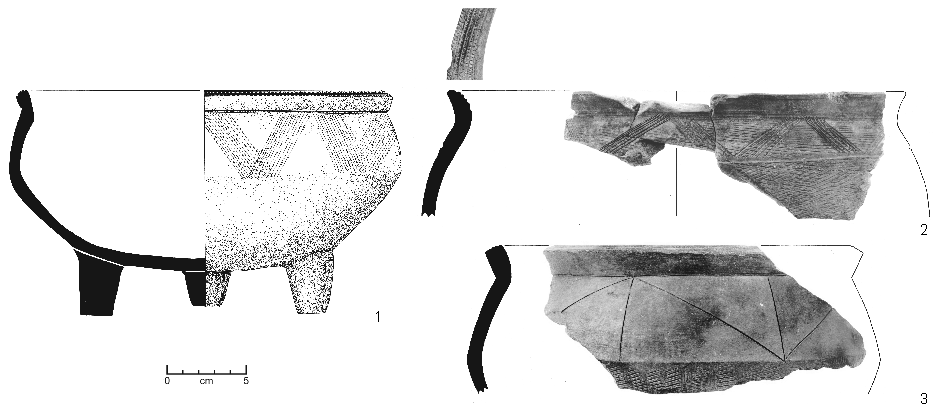
\includegraphics[width=\textwidth]{fig/BKW-Typen.pdf}
\caption{Bokwango-Gruppe: Typvertreter.\\1:~Taf.~2.1; 2:~Taf.~5.1; 3:~Taf.~1.1.}\label{Fig-BKW-Typvertreter}
\end{figure*}

\paragraph{Formen}\hspace{-.5em}|\hspace{.5em}%
Die am häufigsten angetroffene Gefäßform der Bokwango-Gruppe sind bauchige Gefäße ohne ausgearbeiteten Gefäßhals und mit kurzem ausbiegendem Rand (Typ G3; Abb.~\ref{Fig-BKW-Typvertreter}.1,~3). Die eindeutig dieser Gefäßform zugewiesenen Stücke sowie solche, die möglicherweise diesem Typ zugerechnet werden können, machen zusammen fast 84\,\% aller beobachteten Gefäßformen aus. Darüber hinaus wurden lediglich jeweils ein schalenförmiges Gefäß mit konvexer Wandung und einbiegendem Rand (H2) sowie eines mit abknickender Wandung (G2) beobachtet.

Insgesamt konnte bei zwölf GE die Randform beobachtet werden. Die GE der Bokwango-Keramik weisen größtenteils ausbiegende Ränder auf (B; 75\,\%; Abb.~\ref{Fig-BKW-Typvertreter}.1--3), wobei die einfache Variante B1, die bei fünf GE beobachtet wurde, den größten Anteil einnimmt (42\,\%). Daneben konnten noch die kurze Variante B1.1 sowie eine GE mit einem leicht konkaven ausbiegenden Rand beobachtet werden (B2; Abb.~\ref{Fig-BKW-Typvertreter}.2). Parallele (A1) oder einbiegende Ränder (C1) kamen ebenfalls nur in Einzelfällen vor. Über die Hälfte aller Ränder zeigen schräg nach außen abgestrichene Randabschlüsse (M5; 58\,\%; Abb.~\ref{Fig-BKW-Typvertreter}.3), während runde (M1; 17\,\%; Abb.~\ref{Fig-BKW-Typvertreter}.1), spitze (M2; 8\,\%; Abb.~\ref{Fig-BKW-Typvertreter}.2) sowie gerade abgestrichene Randabschlüsse (M3; 8\,\%) deutlich seltener vorkommen. In der Zusammenschau sind kurze, gerade ausbiegende Ränder mit schräg abgestrichener Mündung die bestimmende Randform der Bokwango-Gruppe.

Ein auffälliges Charakteristikum des Bokwango-Stils sind leichte Knicke des Gefäßbauches (Abb.~\ref{Fig-BKW-Typvertreter}.1,~3). Bei 42\,\% der GE, bei denen der entsprechende Bereich erhalten war, wurde ein leichter Bauchknick beobachtet. Die restlichen GE zeigen entweder einen runden Gefäßbauch oder einen abgerundeten Knick im Profil. Die Ausbildung des Gefäßbauches mit einem deutlichen Knick, der auch für die Verzierung der Gefäße eine Begrenzung darstellt, erinnert stark an die Formen der Mokelo-Gruppe (Kap.~\ref{sec:MKL-Gr}). Der Schulterbereich der Bokwango-Gefäße ist regelhaft gerade ausgearbeitet und im Gros der Fälle geht der obere Bauchbereich beziehungsweise die Gefäßschulter direkt in den Rand über (Abb.~\ref{Fig-BKW-Typvertreter}.1,~3). Eine ausgeprägte Halszone wurde bei keiner der GE der Bokwango-Gruppe beobachtet. 

Zwei Schalen des Typs G3 wiesen kleine Standfüßchen auf. Eine entsprechende Bodenform wurde bislang nicht von \textcite[440~Taf.~6]{Wotzka.1995} beschrieben. Eines der Gefäße, das fast vollständig erhalten vorliegt, zeigt drei etwa 35\,mm lange und zirka 25\,mm durchmessende, zylindrische Füße (Abb.~\ref{Fig-BKW-Typvertreter}.1). Im Fall der zweiten, ebenfalls vollständig erhaltenen Schale wurden ebenfalls drei etwa 25\,mm hohe und 20\,mm durchmessende, zylindrische Füße beobachtet (Taf.~1.2). Die beiden Stücken definieren einen neuen Boden-Typ B15 (siehe Kap.~\ref{sec:Bodenform}; Abb.~\ref{fig:Keramik_BodenFormen}). Beide Stücke sind vollständig erhalten und Teil jenes Grundstocks an GE, der für die formale Beschreibung der Stilgruppe herangezogen werden konnte. Da von keiner anderen, der Bokwango-Gruppe zugeordneten GE die Bodenpartie erhalten war, können keine weiterführenden generalisierenden Aussagen zu den Böden dieser Stilgruppe gemacht werden.

\begin{figure*}[p]
	\centering
	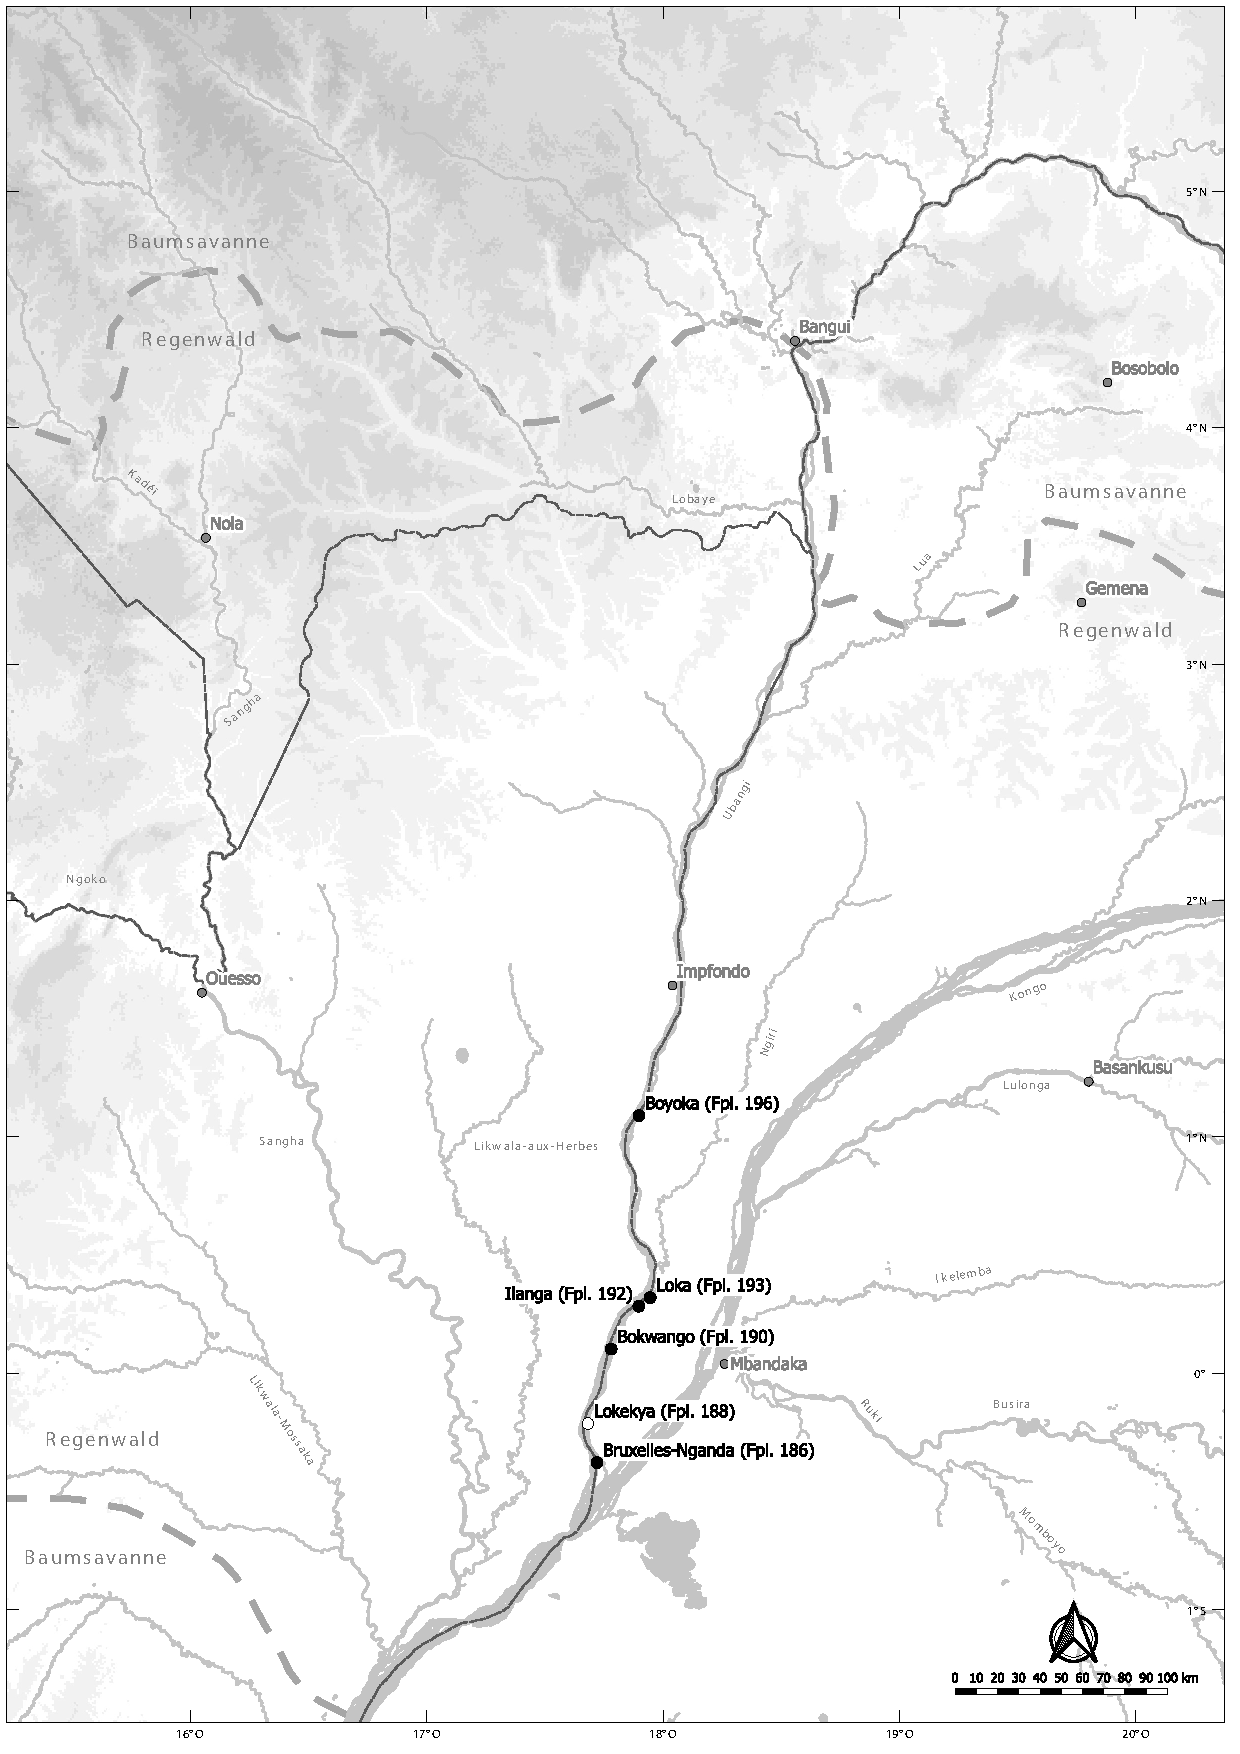
\includegraphics[width=\textwidth]{fig/BKW_Verbreitung.pdf}
	\caption{Bokwango-Gruppe: Verbreitung.}
	\label{Fig-BKW_Verbreitung}
\end{figure*}

\paragraph{Verzierungen}\hspace{-.5em}|\hspace{.5em}%
Die Verzierungen der Gefäße der Bokwango-Gruppe werden von \textit{banfwa-nfwa} (Tab.~\ref{tab:Verzierungselemente}: 08) sowie horizontalen Rillen (Tab.~\ref{tab:Verzierungselemente}: 02.1) bestimmt (Anlage~4\subref{fig:BKW_Verz}). Die Verzierung mit \textit{banfwa-nfwa} findet sich vor allem im Schulter- und Bauchbereich der Gefäße sowie innen am Rand. Sie macht rund 39\,\% aller beobachteten Verzierungen aus. Die horizontalen Rillen, die etwa 23\,\% aller Verzierungselemente ausmachen, finden sich vor allem auf der Innenseite der Ränder sowie außen am Rand. Auf der Schulterpartie der Gefäße finden sich neben \textit{banfwa-nfwa}-Verzierungen häufig großflächige überkreuzte Ritzmuster (Tab.~\ref{tab:Verzierungselemente}: 01.11) oder Bündel aus feinen, winkelförmig laufenden Ritzlinien (Tab.~\ref{tab:Verzierungselemente}: 01.6; Abb.~\ref{Fig-BKW-Typvertreter}.1--3). Die Unterseiten der Gefäße sind häufig unverziert oder weisen flächiges \textit{banfwa-nfwa} auf (Abb.~\ref{Fig-BKW-Typvertreter}.2--3).

\paragraph{Datierung}\hspace{-.5em}|\hspace{.5em}%
Für die Keramik der Bokwango-Gruppe liegen keine absoluten Datierungen vor. Das beobachtete Spektrum an Formen und Verzierungen lässt jedoch Ähnlichkeiten zu verschiedenen Stilen des Inneren Kongobeckens erkennen \parencite{Wotzka.1995}. Länglich gezogene Schulterpartien sowie leichte Absätze im oberen Schulterbereich (Abb.~\ref{Fig-BKW-Typvertreter}.2) lassen sich auch bei Gefäßen aus Mbandaka (Fpl.~10) beobachten, die dem gleichnamigen Stil zugeordnet sind (ebd. 139--143, 447 Taf.~13.1--5). Eine sehr ähnliche Grundform kann auch bei einem der Nkile-Gruppe (ebd. 144--150) zugerechneten Gefäß aus Bamanya (Fpl.~12) beobachtet werden (ebd. 450 Taf.~16.6). Ein Gefäß der Lokondola-Gruppe aus Nkile (Fpl.~17) weist einen einfach ausbiegenden Rand mit schräg abgestrichener Randlippe, der in eine nur leicht geschweifte Gefäßschulter übergeht, auf (ebd. 84--89, 463 Taf.~29.14). Entsprechungen dafür lassen sich bei Gefäßen der Bokwango-Gruppe beobachten (Abb.~\ref{Fig-BKW-Typvertreter}.3). Eine vergleichbare Gliederung der verzierten Gefäßbereiche in ein Oberteil mit Ritzverzierung und ein Unterteil mit \textit{banfwa-nfwa} ist für der Botendo-Gruppe (ebd. 150--158) zugerechnete Schalen vom eponymen Fundort charakteristisch (Fpl.~25; ebd. 482 Taf.~48.5--7). Ein dem Stil Botendo oder Ikenge \parencite[siehe][]{Eggert.1980c} zuordenbares Gefäß aus Boangi \parencite[Fpl.~61;][508 Taf.~74.11]{Wotzka.1995} weist ebenfalls schwache Parallelen zu den leicht bauchigen und eher spärlich verzierten Gefäßen der Bokwango-Gruppe auf (Abb.~\ref{Fig-BKW-Typvertreter}.1). Mit Ausnahme der Parallele zu dem aus Nkile bekannten Gefäß der Lokondola-Gruppe (Fpl.~17; ebd. 463 Taf.~29.14) datieren alle Vergleichsfunde aus dem Inneren Kongobecken in das 2.~Jt. n.~Chr.

Mit Bezug auf die Stilgruppen des nordwestlichen Kongobeckens zeigt sich in der deutlichen Profilierung der Gefäße der Bokwango-Gruppe ein schwacher Bezug zu der am mittleren \mbox{Ubangi} verbreiteten Mokelo-Keramik (Kap.~\ref{sec:MKL-Gr}). Mit Blick auf die -- wenn auch losen -- Vergleiche für die Bokwango-Keramik aus dem Inneren Kongobecken ließe sich die chronologische Stellung dieser Stilgruppe grob auf das 2.~Jt. n.~Chr. eingrenzen. Es muss offenbleiben, bis zu welchem Grad die Keramik der Bokwango-Gruppe eine eigenständige keramische Entwicklung des nordwestlichen Kongobeckens widerspiegelt. In der Zusammenschau kann zumindest auf hypothetischer Ebene die Zugehörigkeit der Bokwango-Keramik zu den Stilgruppen der \enquote{West-Tradition der Äquator-Co-Tradition} (ebd. 221\,f.) des Inneren Kongobeckens postuliert werden (Abb.~\ref{fig:Chronologiesystem}).

\paragraph{Verbreitung}\hspace{-.5em}|\hspace{.5em}%
Das Fundmaterial der Bokwango-Gruppe beschränkt sich auf fünf Fundstellen entlang des unteren \mbox{Ubangi}, wobei das \textit{Nganda}\footnote{\textit{Nganda} bezeichnet ein vornehmlich saisonal genutztes Fischercamp, das stellenweise aus Pfahlbauten oder wurtenartigen Anlagen besteht (\textsc{Wotzka} 1995: 19 Anm.~6).\label{ftn:Nganda}} Bruxelles (Fpl.~186) im Bereich der Mündung des \mbox{Ubangi} in den Kongo die südlichste und Boyoka (Fpl.~196) die nördlichste Fundstelle ist (Abb.~\ref{Fig-BKW_Verbreitung}). Aus Lokekya (Fpl.~188) liegt eine weitere mögliche GE der Bokwango-Gruppe vor. Keines der dieser Gruppe zugewiesenen Stücke stammt aus einem ergrabenen Befund, alle GE fanden sich in Absammlungen von rezenten Dorfflächen.